% !TeX program = xelatex
\documentclass[a4paper,10pt]{article}

% ============================================================================
% កញ្ចប់បណ្ណាល័យ (Packages) – តាមលំនាំ NGS Preah Krasang (ls_plan.tex)
% បរិបទ៖ គ្មានស្លាយ LCD និងគ្មានម៉ាស៊ីនគិតលេខ — ប្រើសន្លឹកកិច្ចការសិស្ស (ស-ខ្មៅ) និងក្ដារខៀនជាគោល
% ============================================================================
\usepackage[a4paper, left=0.95cm, right=0.95cm, top=0.85cm, bottom=0.92cm, footskip=0.52cm]{geometry}
\usepackage{amsmath}
\usepackage{unicode-math}
\usepackage{fontspec}
\usepackage{array, longtable, multirow, colortbl}
\usepackage[table]{xcolor}
\usepackage{enumitem}
\usepackage{pifont}
\usepackage{fancyhdr}
\usepackage{tikz}
\usetikzlibrary{calc, arrows.meta, angles, quotes, decorations.markings, decorations.pathreplacing, patterns, babel}

\makeatletter
\let\@expl@@@mark@update@singlecol@structures@@\relax
\makeatother

\providecommand{\NGSFindFonts}{%
  \IfFileExists{C:/Windows/Fonts/cambria.ttc}{%
    \def\NGSSysPath{C:/Windows/Fonts/}%
    \def\NGSUserPath{C:/Users/KIT/AppData/Local/Microsoft/Windows/Fonts/}%
  }{%
    \IfFileExists{./fonts/KhmerOSsiemreap.ttf}{\def\NGSSysPath{./fonts/}\def\NGSUserPath{./fonts/}}{%
    \IfFileExists{../fonts/KhmerOSsiemreap.ttf}{\def\NGSSysPath{../fonts/}\def\NGSUserPath{../fonts/}}{%
    \IfFileExists{../../fonts/KhmerOSsiemreap.ttf}{\def\NGSSysPath{../../fonts/}\def\NGSUserPath{../../fonts/}}{%
    \IfFileExists{../../../fonts/KhmerOSsiemreap.ttf}{\def\NGSSysPath{../../../fonts/}\def\NGSUserPath{../../../fonts/}}{%
    \IfFileExists{../../../../fonts/KhmerOSsiemreap.ttf}{\def\NGSSysPath{../../../../fonts/}\def\NGSUserPath{../../../../fonts/}}{%
    \IfFileExists{../../../../../fonts/KhmerOSsiemreap.ttf}{\def\NGSSysPath{../../../../../fonts/}\def\NGSUserPath{../../../../../fonts/}}{%
    \IfFileExists{../../../../../../fonts/KhmerOSsiemreap.ttf}{\def\NGSSysPath{../../../../../../fonts/}\def\NGSUserPath{../../../../../../fonts/}}{%
      \def\NGSSysPath{../../../../../../../fonts/}\def\NGSUserPath{../../../../../../../fonts/}%
    }}}}}}}%
  }%
}
\NGSFindFonts

\setmathfont[Path={\NGSSysPath}, FontIndex=1, Scale=1.02]{cambria.ttc}
\defaultfontfeatures{Ligatures=TeX}

\setmainfont[
  Path={\NGSUserPath}, Extension=.ttf, Script=Khmer,
  BoldFont={KhmerOSsiemreap}, BoldFeatures={FakeBold=1.8},
  ItalicFont={KhmerOSsiemreap}, ItalicFeatures={FakeSlant=0.25},
  BoldItalicFont={KhmerOSsiemreap}, BoldItalicFeatures={FakeBold=1.8, FakeSlant=0.25}
]{KhmerOSsiemreap}

\newfontfamily\muol[Path={\NGSUserPath}, Extension=.ttf, Script=Khmer]{KhmerOSmuollight}
\newfontfamily\TimesEn[Path={\NGSSysPath}, Extension=.ttf, Scale=1.00, BoldFont={timesbd}, ItalicFont={timesi}, BoldItalicFont={timesbi}]{times}
\newfontfamily\NagaBold[Path={\NGSUserPath}, Extension=.ttf]{AKbalthom Naga Bold}
\newfontfamily\CalibriFont[Path={\NGSSysPath}, Extension=.ttf]{calibri}
\newfontfamily\Tacteing[Path={\NGSUserPath}]{TACTENG.TTF}
\newfontfamily\CourierBullet[Path={\NGSSysPath}, Extension=.ttf]{cour}
\newcommand{\wcirc}{{\CourierBullet\fontsize{9.5pt}{11pt}\selectfont o}}

\XeTeXlinebreaklocale "km"
\XeTeXlinebreakskip = 0pt plus 1pt minus 0.1pt

\definecolor{stepgray}{HTML}{D9D9D9}
\definecolor{headgray}{HTML}{F2F2F2}
\definecolor{boxgray}{HTML}{D9D9D9}
\definecolor{darkred}{HTML}{C00000}
\definecolor{red5e}{HTML}{FF0000}

\pagestyle{fancy}
\fancyhf{}
\renewcommand{\headrulewidth}{0pt}
\fancyfoot[R]{\CalibriFont\fontsize{11pt}{13pt}\selectfont\thepage}

\setlength{\parindent}{0pt}
\setlength{\parskip}{0pt}
\setlength{\tabcolsep}{3.8pt}

\newcolumntype{L}[1]{>{\raggedright\arraybackslash}p{#1}}
\newcolumntype{C}[1]{>{\centering\arraybackslash}p{#1}}

\newcommand{\en}[1]{{\TimesEn #1}}
\newcommand{\enbf}[1]{{\TimesEn\textbf{#1}}}
\newcommand{\unit}[1]{\,\text{\en{#1}}}
\newcommand{\fiveE}[1]{{\NagaBold\fontsize{9.5pt}{13pt}\selectfont\textcolor{red5e}{#1}}}
\newcommand{\timenote}[1]{\textcolor{darkred}{\textit{#1}}}
\newcommand{\redsub}[1]{\textcolor{darkred}{#1}}
\newcommand{\graybox}[1]{\colorbox{boxgray}{\strut\hspace{2pt}#1\hspace{2pt}}}
\newcommand{\ditem}{\tikz[baseline=-0.5ex]\fill (0,0.42ex) -- (0.42ex,0) -- (0,-0.42ex) -- (-0.42ex,0) -- cycle;\hspace{0.3em}}
\newcommand{\cnum}[1]{{\fontsize{10.5pt}{12pt}\selectfont\ding{\numexpr181+#1\relax}}\hspace{0.15em}}
\newcommand{\cfig}[1]{\par\vspace{3pt}{\centering #1\par}\vspace{3pt}}
\newcommand{\stepheader}[1]{\multicolumn{3}{|c|}{\cellcolor{stepgray}\muol #1} \\* \noalign{\hrule height 0.4pt}}
\newcommand{\khmflourish}{{\Tacteing\fontsize{36pt}{14pt}\selectfont\raisebox{-5pt}{3}}}

% ============================================================================
% ម៉ាក្រូគូសរូប TikZ ស-ខ្មៅ ១០០% សម្រាប់មេរៀន ៣.១.២ លក្ខណៈនៃសមាមាត្រស្រប (PROP2)
% ============================================================================

% ១. E1 Engage: អង្ករកាកបាទក្រហម 320 kg និងចតុកោណកែងសមាមាត្រ (ទំ.២៨-២៩)
\newcommand{\figEngagePROPB}{%
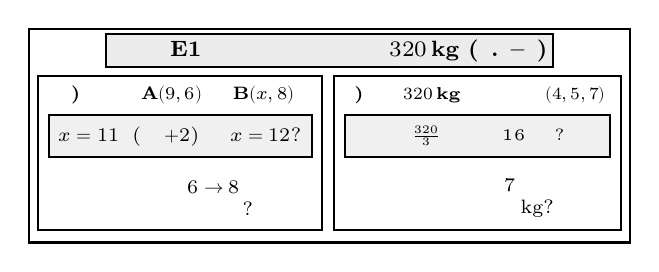
\begin{tikzpicture}[x=0.96cm, y=0.92cm, every node/.style={font=\scriptsize, text=black}]
  \draw[black, line width=0.95pt] (0,0) rectangle (7.95,2.95);
  \node[fill=gray!15, draw=black, line width=0.6pt, inner sep=2pt, font=\footnotesize\bfseries] at (3.975,2.65) {បេសកកម្ម \en{E1}៖ ចតុកោណកែងសមាមាត្រ និងអង្ករ $320\unit{kg}$ (ទំ.២៨–២៩)};

  \draw[black, line width=0.8pt] (0.12,0.18) rectangle (3.88,2.30);
  \node[font=\fontsize{6.5pt}{8.5pt}\selectfont\bfseries] at (2.00,2.04) {១) ចតុកោណកែង \en{A}$(9,6)$ និង \en{B}$(x,8)$};
  \draw[black, line width=0.75pt, fill=gray!12] (0.26,1.18) rectangle (3.74,1.76);
  \node at (2.00,1.47) {$x = 11$ \;(បូក $+2$) \;ឬ\; $x = 12$?};
  \node[align=center] at (2.00,0.62) {បើទទឹងកើនពី $6 \to 8$\\តើបណ្ដោយត្រូវស្មើប៉ុន្មាន?};

  \draw[black, line width=0.8pt] (4.04,0.18) rectangle (7.83,2.30);
  \node[font=\fontsize{6.2pt}{8pt}\selectfont\bfseries] at (5.935,2.04) {២) អង្ករ $320\unit{kg}$ ចែក ៣ គ្រួសារ $(4,5,7)$};
  \draw[black, line width=0.75pt, fill=gray!12] (4.18,1.18) rectangle (7.69,1.76);
  \node[font=\fontsize{5.9pt}{7.6pt}\selectfont] at (5.935,1.47) {ចែក $\frac{320}{3}$ \;ឬ\; ចែកតាម $16$ ចំណែក?};
  \node[align=center] at (5.935,0.62) {តើគ្រួសារមានគ្នា $7$ នាក់\\ត្រូវទទួលបានប៉ុន្មាន $\unit{kg}$?};
\end{tikzpicture}}

% ២. E2 POE 1: ចតុកោណកែង A(9,6), B(x,8), C(15,y) និងស្ពានតួចុង-តួមធ្យម (ទំ.២៨-២៩)
\newcommand{\figRectsPROPB}{%
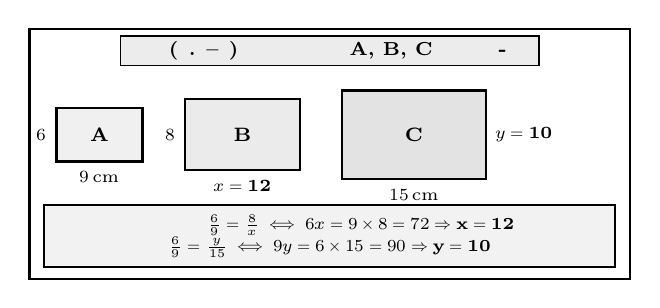
\begin{tikzpicture}[x=0.96cm, y=0.92cm, every node/.style={font=\scriptsize, text=black}]
  \draw[black, line width=0.95pt] (0,0) rectangle (7.95,3.45);
  \node[fill=gray!15, draw=black, line width=0.6pt, inner sep=2pt, font=\fontsize{6.8pt}{8.5pt}\selectfont\bfseries] at (3.975,3.15) {គំរូ ១ (ទំ.២៨–២៩)៖ ចតុកោណកែងសមាមាត្រ \en{A, B, C} និងគុណតួចុង-មធ្យម};

  % Rect A
  \draw[black, line width=0.85pt, fill=gray!12] (0.36,1.62) rectangle (1.50,2.36);
  \node at (0.93,1.99) {\textbf{\en{A}}};
  \node[below, font=\fontsize{6.2pt}{7.8pt}\selectfont] at (0.93,1.62) {$9\unit{cm}$};
  \node[left, font=\fontsize{6.2pt}{7.8pt}\selectfont] at (0.36,1.99) {$6$};

  % Rect B
  \draw[black, line width=0.85pt, fill=gray!16] (2.06,1.50) rectangle (3.58,2.48);
  \node at (2.82,1.99) {\textbf{\en{B}}};
  \node[below, font=\fontsize{6.2pt}{7.8pt}\selectfont] at (2.82,1.50) {$x = \mathbf{12}$};
  \node[left, font=\fontsize{6.2pt}{7.8pt}\selectfont] at (2.06,1.99) {$8$};

  % Rect C
  \draw[black, line width=0.85pt, fill=gray!22] (4.14,1.38) rectangle (6.04,2.60);
  \node at (5.09,1.99) {\textbf{\en{C}}};
  \node[below, font=\fontsize{6.2pt}{7.8pt}\selectfont] at (5.09,1.38) {$15\unit{cm}$};
  \node[right, font=\fontsize{6.2pt}{7.8pt}\selectfont] at (6.04,1.99) {$y = \mathbf{10}$};

  % Cross-product formula box on bottom (2 crisp lines)
  \draw[black, line width=0.75pt, fill=gray!10] (0.20,0.16) rectangle (7.75,1.02);
  \node[align=center, font=\fontsize{6.1pt}{7.8pt}\selectfont] at (3.975,0.59) {\textbf{លក្ខណៈទី ១៖} $\frac{6}{9} = \frac{8}{x} \iff 6x = 9\times 8 = 72 \Rightarrow \mathbf{x=12}$\\$\frac{6}{9} = \frac{y}{15} \iff 9y = 6\times 15 = 90 \Rightarrow \mathbf{y=10}$};
\end{tikzpicture}}

% ៣. E4 Singapore Bar Model: អង្ករកាកបាទក្រហម 320 kg (4 + 5 + 7 = 16 ចំណែក, ទំ.២៩-៣០)
\newcommand{\figBarModelPROPB}{%
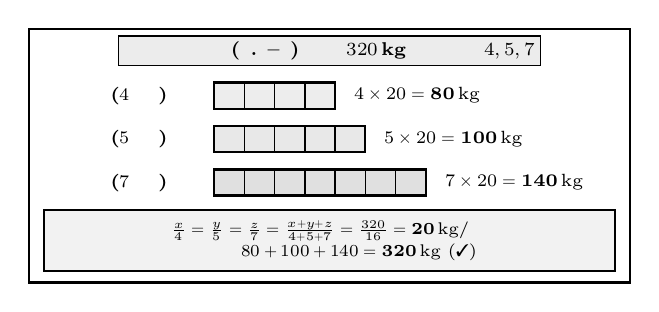
\begin{tikzpicture}[x=0.96cm, y=0.92cm, every node/.style={font=\scriptsize, text=black}]
  \draw[black, line width=0.95pt] (0,0) rectangle (7.95,3.50);
  \node[fill=gray!15, draw=black, line width=0.6pt, inner sep=2pt, font=\fontsize{6.7pt}{8.5pt}\selectfont\bfseries] at (3.975,3.20) {គំរូរបារភាគស្មើគ្នា (ទំ.២៩–៣០)៖ អង្ករ $320\unit{kg}$ ចែកតាមសមាជិក $4, 5, 7$};

  % Family 1: 4 units
  \node[anchor=west, font=\fontsize{6.4pt}{8pt}\selectfont] at (0.18,2.58) {\textbf{គ្រួសារទី១ ($4$ នាក់)៖}};
  \draw[black, line width=0.8pt, fill=gray!14] (2.45,2.40) rectangle (4.05,2.76);
  \foreach \k in {1,2,3} {\draw[black, line width=0.5pt] ({2.45+0.40*\k},2.40) -- ({2.45+0.40*\k},2.76);}
  \node[anchor=west, font=\fontsize{6.4pt}{8pt}\selectfont] at (4.18,2.58) {$4\times 20 = \mathbf{80\unit{kg}}$};

  % Family 2: 5 units
  \node[anchor=west, font=\fontsize{6.4pt}{8pt}\selectfont] at (0.18,1.98) {\textbf{គ្រួសារទី២ ($5$ នាក់)៖}};
  \draw[black, line width=0.8pt, fill=gray!18] (2.45,1.80) rectangle (4.45,2.16);
  \foreach \k in {1,2,3,4} {\draw[black, line width=0.5pt] ({2.45+0.40*\k},1.80) -- ({2.45+0.40*\k},2.16);}
  \node[anchor=west, font=\fontsize{6.4pt}{8pt}\selectfont] at (4.58,1.98) {$5\times 20 = \mathbf{100\unit{kg}}$};

  % Family 3: 7 units
  \node[anchor=west, font=\fontsize{6.4pt}{8pt}\selectfont] at (0.18,1.38) {\textbf{គ្រួសារទី៣ ($7$ នាក់)៖}};
  \draw[black, line width=0.8pt, fill=gray!24] (2.45,1.20) rectangle (5.25,1.56);
  \foreach \k in {1,2,3,4,5,6} {\draw[black, line width=0.5pt] ({2.45+0.40*\k},1.20) -- ({2.45+0.40*\k},1.56);}
  \node[anchor=west, font=\fontsize{6.4pt}{8pt}\selectfont] at (5.38,1.38) {$7\times 20 = \mathbf{140\unit{kg}}$};

  % Bottom summary (2 crisp lines)
  \draw[black, line width=0.75pt, fill=gray!10] (0.20,0.16) rectangle (7.75,1.00);
  \node[align=center, font=\fontsize{6.1pt}{7.8pt}\selectfont] at (3.975,0.58) {$\frac{x}{4}=\frac{y}{5}=\frac{z}{7}=\frac{x+y+z}{4+5+7}=\frac{320}{16}=\mathbf{20\unit{kg}\text{/នាក់}}$\\ផ្ទៀងផលបូក៖ $80+100+140 = \mathbf{320\unit{kg}}$ (\ding{51})};
\end{tikzpicture}}

% ៤. E5 Diagnostic Options A-D
\newcommand{\figExitCardsPROPB}{%
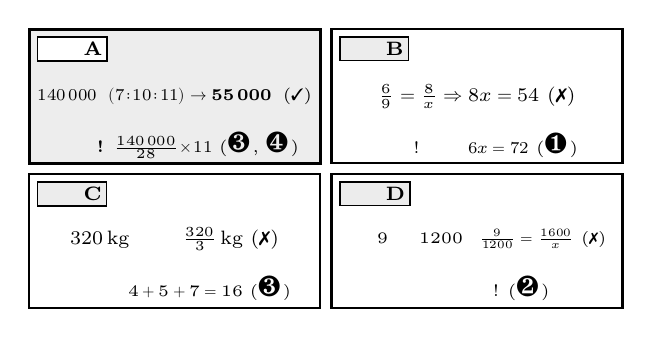
\begin{tikzpicture}[x=0.96cm, y=0.92cm, every node/.style={font=\scriptsize, text=black}]
  \draw[black, line width=1.1pt, fill=gray!14] (0,2.00) rectangle (3.85,3.85);
  \node[anchor=north west, fill=white, draw=black, line width=0.6pt, inner sep=1.8pt] at (0.10,3.75) {\textbf{ជម្រើស \en{A}}};
  \node[font=\fontsize{6.0pt}{7.8pt}\selectfont] at (1.925,2.92) {$140\,000\text{៛}$ $(7\!:\!10\!:\!11) \to \mathbf{55\,000\text{៛}}$ (\ding{51})};
  \node[font=\fontsize{6.0pt}{7.8pt}\selectfont] at (1.925,2.25) {\textbf{ត្រឹមត្រូវ!} $\frac{140\,000}{28}\!\times\! 11$ (\cnum{3}, \cnum{4})};

  \draw[black, line width=0.9pt] (4.00,2.00) rectangle (7.85,3.85);
  \node[anchor=north west, fill=gray!15, draw=black, line width=0.6pt, inner sep=1.8pt] at (4.10,3.75) {\textbf{ជម្រើស \en{B}}};
  \node at (5.925,2.92) {$\frac{6}{9} = \frac{8}{x} \Rightarrow 8x = 54$ (\ding{55})};
  \node[font=\fontsize{6.0pt}{7.8pt}\selectfont] at (5.925,2.25) {គុណខុសគូ! ត្រូវជា $6x = 72$ (\cnum{1})};

  \draw[black, line width=0.9pt] (0,0) rectangle (3.85,1.85);
  \node[anchor=north west, fill=gray!15, draw=black, line width=0.6pt, inner sep=1.8pt] at (0.10,1.75) {\textbf{ជម្រើស \en{C}}};
  \node at (1.925,0.95) {$320\unit{kg}$ ចែកស្មើ $\frac{320}{3}\unit{kg}$ (\ding{55})};
  \node[font=\fontsize{5.8pt}{7.5pt}\selectfont] at (1.925,0.28) {ភ្លេចបូកសមាជិក $4+5+7=16$ (\cnum{3})};

  \draw[black, line width=0.9pt] (4.00,0) rectangle (7.85,1.85);
  \node[anchor=north west, fill=gray!15, draw=black, line width=0.6pt, inner sep=1.8pt] at (4.10,1.75) {\textbf{ជម្រើស \en{D}}};
  \node[font=\fontsize{5.8pt}{7.5pt}\selectfont] at (5.925,0.95) {ក្រូច $9$ ថ្លៃ $1200\text{៛}$៖ $\frac{9}{1200}=\frac{1600}{x}$ (\ding{55})};
  \node[font=\fontsize{6.0pt}{7.8pt}\selectfont] at (5.925,0.28) {ដាក់ឯកតាបញ្ច្រាសជួរ! (\cnum{2})};
\end{tikzpicture}}

\begin{document}
\fontsize{10pt}{15.2pt}\selectfont

% -------------------- ក្បាលកិច្ចតែងការ --------------------
\begin{center}
  {\muol\fontsize{11pt}{16pt}\selectfont ព្រះរាជាណាចក្រកម្ពុជា}\\[2pt]
  {\muol\fontsize{10pt}{15pt}\selectfont ជាតិ សាសនា ព្រះមហាក្សត្រ}\\[1pt]
  \khmflourish
\end{center}

\vspace{-24pt}
{\muol\fontsize{9.5pt}{12.5pt}\selectfont
មន្ទីរអប់រំ យុវជន និងកីឡា ខេត្តកំពង់ធំ\\
ការិយាល័យអប់រំ យុវជន និងកីឡា ស្រុកកំពង់ស្វាយ\\
អនុវិទ្យាល័យព្រះក្រសាំង}

\vspace{1pt}
\begin{center}
  {\muol\fontsize{10pt}{14pt}\selectfont កិច្ចតែងការបង្រៀន}
\end{center}
\vspace{0pt}

% -------------------- ព័ត៌មានទូទៅ --------------------
{\renewcommand{\arraystretch}{0.98}
\hspace*{3.1cm}%
\begin{tabular}{@{}l l L{11.0cm}@{}}
  - \hspace{0.35cm} មុខវិជ្ជា & : & គណិតវិទ្យា ថ្នាក់ទី៨ (ពីជគណិត) \\
  - \hspace{0.35cm} ចំណងជើងមេរៀន & : & មេរៀនទី៣៖ ទំហំសមាមាត្រ និងភាគរយ \\
  - \hspace{0.35cm} ចំណងជើងរង & : & ១.២. លក្ខណៈនៃសមាមាត្រស្រប (ទំ.២៨–៣០ និងលំហាត់ \#1, \#2, \#4, \#5ក, \#11, \#12 ទំ.៤០–៤១) \\
  - \hspace{0.35cm} រយៈពេល & : & ១ ម៉ោងសិក្សា (៥០ នាទី) \\
  - \hspace{0.35cm} បង្រៀនដោយ & : & ហុក ប៊ុនថែន \\
  - \hspace{0.35cm} កាលបរិច្ឆេទ & : & ថ្ងៃព្រហស្បតិ៍ ទី២៦ ខែវិច្ឆិកា ឆ្នាំ២០២៦ \\
\end{tabular}

\vspace{2pt}

% -------------------- I. វត្ថុបំណង --------------------
\textbf{I.} {\muol វត្ថុបំណង}\\[1pt]
\hspace*{0.55cm}%
\begin{tabular}{@{}l l L{14.2cm}@{}}
  \wcirc \hspace{0.25cm} វិជ្ជាសម្បទា & : & សិស្សប្រាប់លក្ខណៈទាំងពីរនៃសមាមាត្រស្រប គឺផលគុណតួចុងស្មើផលគុណតួមធ្យម ($x_2 y_1 = x_1 y_2$) និងលក្ខណៈផលបូកផលធៀបស្មើគ្នា ($\frac{y_1}{x_1}=\frac{y_2}{x_2}=\frac{y_3}{x_3}=\frac{y_1+y_2+y_3}{x_1+x_2+x_3}$) ។ \\
  \wcirc \hspace{0.25cm} បំណិនសម្បទា & : & សិស្សគណនាតួមិនស្គាល់ក្នុងសមាមាត្រ និងដោះស្រាយចំណោទបែងចែកបរិមាណសមាមាត្រតាមចំនួនចំណែក (អង្ករកាកបាទក្រហម ផ្លែក្រូច និងប្រាក់ចែកកូន ទំ.២៨–៣០) លើសន្លឹកកិច្ចការ ។ \\
  \wcirc \hspace{0.25cm} ចរិយាសម្បទា & : & សិស្សមានភាពយុត្តិធម៌ និងម៉ត់ចត់ក្នុងការបែងចែកបរិមាណតាមសមាមាត្រ ព្រមទាំងមានទម្លាប់ផ្ទៀងផ្ទាត់ផលបូកត្រឡប់ជានិច្ច ។ \\
\end{tabular}

\vspace{2pt}

% -------------------- II. សម្ភារៈឧបទេស --------------------
\textbf{II.} {\muol សម្ភារៈឧបទេស}\\[1pt]
\hspace*{0.55cm}$\bullet$ \hspace{0.35cm} សៀវភៅសិក្សាគោលគណិតវិទ្យាថ្នាក់ទី៨ (ទំ.២៨–៣០, ៤០–៤១) ក្ដារខៀន ដីស និងសន្លឹកកិច្ចការសិស្ស ស-ខ្មៅ (\en{Worksheet\_PROP2} ទំព័រ ១–២ គ្មានស្លាយ \en{LCD})

\vspace{2pt}

% -------------------- III. វិធីសាស្រ្តបង្រៀន --------------------
\textbf{III.} {\muol វិធីសាស្រ្តបង្រៀន}\\[1pt]
\hspace*{0.45cm}%
\begin{tabular}{@{}l l L{14.85cm}@{}}
  $\bullet$ \hspace{0.25cm} គោលវិធី & : & សិស្សមជ្ឈមណ្ឌល (បង្រៀនតាមសន្លឹកកិច្ចការស៊ើបអង្កេត និងក្ដារខៀន គ្មាន \en{LCD}) \\
  $\bullet$ \hspace{0.25cm} យុទ្ធវិធីបង្រៀន & : & គំរូ \en{5Es} រួមបញ្ចូលស្ពានតួចុង-តួមធ្យមមានស្លាកឯកតា និងគំរូរបារភាគស្មើគ្នាសិង្ហបុរី (\en{Singapore Bar-Model Allocation}) \\
\end{tabular}
}

\vspace{2pt}

% -------------------- IV. ដំណើរការបង្រៀន --------------------
\textbf{IV.} {\muol ដំណើរការបង្រៀន}

\vspace{1pt}

\renewcommand{\arraystretch}{1.15}
\begin{longtable}{|L{5.50cm}|L{7.90cm}|L{4.80cm}|}
\hline
\rowcolor{headgray}
\multicolumn{1}{|c|}{\muol សកម្មភាពគ្រូ} &
\multicolumn{1}{c|}{\muol ខ្លឹមសារមេរៀន} &
\multicolumn{1}{c|}{\muol សកម្មភាពសិស្ស} \\
\hline
\endfirsthead
\hline
\endhead
\hline
\endfoot
\hline
\endlastfoot

% ==================== ជំហានទី១ (2min) ====================
\stepheader{ជំហានទី១ \enbf{(}រដ្ឋបាលថ្នាក់\enbf{)}}
$\bullet$ ពិនិត្យអវត្តមាន អនាម័យ និងសណ្ដាប់ធ្នាប់ថ្នាក់រៀន
&
$\bullet$ រដ្ឋបាលថ្នាក់ និងការរៀបចំដៃគូសិក្សា
&
$\circ$ ប្រធានថ្នាក់រាយការណ៍អវត្តមាន \\[3pt]

$\bullet$ ចែក \textbf{សន្លឹកកិច្ចការសិស្ស (\en{Worksheet\_PROP2})} ម្នាក់ ១ សន្លឹក (ផ្កាប់ទុកសិន)
&
$\bullet$ សន្លឹកកិច្ចការសិស្ស ស-ខ្មៅ (\en{Worksheet\_PROP2} ទំព័រ ១–២)
&
$\circ$ ទទួលសន្លឹកកិច្ចការ និងត្រៀមសម្ភារៈសរសេរ \\
\hline

% ==================== ជំហានទី២ (9min: <=3 + 3 + E1 3) ====================
\stepheader{ជំហានទី២ \enbf{(}កិច្ចការផ្ទះ \enbf{+} ទំនាក់ទំនងមេរៀនថ្មី\enbf{)}}
\ditem \textbf{កំណែកិច្ចការផ្ទះ ($\le 3\unit{min}$)} \timenote{(កុំសរសេរវែង)} \par
$\bullet$ ហៅសិស្ស ២ នាក់ឡើងសរសេរចម្លើយលំហាត់ \#6ក, \#7 និង \#10 (ទំ.៤០–៤១) លើក្ដារខៀន
&
{\centering\redsub{កំណែកិច្ចការផ្ទះមេរៀន ១.១ (ទំ.៤០–៤១ \#6, \#7, \#10)}\par} \par
$\bullet$ \textbf{\#6៖} ពិនិត្យផលធៀបថេរ $\frac{y}{x} = a$ ដើម្បីសម្រេចថាសមាមាត្រស្រប \par
$\bullet$ \textbf{\#7 និង \#10៖} កំណត់មេគុណសមាមាត្រ $a$ និងគណនាតម្លៃតាម $y = ax$
&
$\circ$ ផ្ទៀងផ្ទាត់ និងកែតម្រូវចម្លើយក្នុងសៀវភៅកិច្ចការផ្ទះ \\[3pt]

\ditem \textbf{រំលឹកមេរៀនទាក់ទង (3min)} \par
$\bullet$ សួររហ័ស៖ បើ $y$ សមាមាត្រស្របនឹង $x$ តើផលធៀប $\dfrac{y_1}{x_1}$ និង $\dfrac{y_2}{x_2}$ មានទំនាក់ទំនងដូចម្ដេចនឹងមេគុណ $a$?
&
{\centering\redsub{រំលឹកនិយមន័យផលធៀបថេរនៃសមាមាត្រស្រប}\par} \par
$\bullet$ ដោយ $\dfrac{y_1}{x_1} = a$ និង $\dfrac{y_2}{x_2} = a \implies \dfrac{y_1}{x_1} = \dfrac{y_2}{x_2}$ (ស្មើគ្នា!)
&
$\circ$ ឆ្លើយរហ័សថាផលធៀបទាំងពីរស្មើគ្នាព្រោះស្មើនឹង $a$ ដូចគ្នា \\[3pt]

\fiveE{E1 - Engage (3min)} \timenote{(កុំទាន់ផ្ដល់ចម្លើយ)} \par
\ditem \textbf{«បេសកកម្មអង្ករកាកបាទក្រហម $320\unit{kg}$ និងចតុកោណកែងសមាមាត្រ»} \par
$\bullet$ ឱ្យសិស្សបើកសន្លឹកកិច្ចការទំព័រ ១ គូសធីកទស្សន៍ទាយលើសំណួរ ២
&
{\centering\redsub{បេសកកម្ម E1៖ អន្ទាក់បូកបន្ថែម និងអន្ទាក់ចែកស្មើ}\par} \par
$\bullet$ \textbf{សំណួរ ១ (ទំ.២៨)៖} ចតុកោណកែងសមាមាត្រ \en{A}$(9,6)$ និង \en{B}$(x,8)$ — តើ $x=11$ ឬ $x=12$? \par
$\bullet$ \textbf{សំណួរ ២ (ទំ.២៩)៖} អង្ករ $320\unit{kg}$ ចែកតាមសមាជិក ៣ គ្រួសារ $(4,5,7)$ — តើគ្រួសារ $7$ នាក់បានប៉ុន្មាន $\unit{kg}$?
&
$\circ$ គូសធីកទស្សន៍ទាយលើសន្លឹកកិច្ចការទំព័រ ១ \\[3pt]

&
\cfig{\figEngagePROPB}
& \\[3pt]

$\bullet$ ស្រង់ចំនួនដៃសិស្សកត់លើក្ដារខៀន (មិនទាន់ប្រាប់ចម្លើយត្រូវ)
&
$\bullet$ ស្ថិតិទស្សន៍ទាយ៖ $x=11$ ទល់នឹង $x=12$ ; ចែកស្មើ $\frac{320}{3}$ ទល់នឹង ចែកតាម $16$ នាក់
&
$\circ$ លើកដៃបង្ហាញការទស្សន៍ទាយ \\
\hline

% ==================== ជំហានទី៣ (17min: E2 11m + E3 6m) ====================
\stepheader{ជំហានទី៣ \enbf{(}ខ្លឹមសារមេរៀនថ្មី\enbf{)}}
\fiveE{E2 - Explore (11min)} \par
$\bullet$ សរសេរចំណងជើងរងលើក្ដារខៀន
&
\textbf{១.២. លក្ខណៈនៃសមាមាត្រស្រប} (សៀវភៅពុម្ព ទំ.២៨–៣០)
&
$\circ$ កត់ចំណងជើងចូលសៀវភៅ \\[3pt]

\ditem \textbf{សកម្មភាព ១៖ ស្ពានតួចុង-តួមធ្យមលើចតុកោណកែង \en{POE 1} (6min, ផ្នែកទី១-ក)} \par
$\bullet$ ឱ្យដៃគូបំបាត់ភាគបែងនៃ $\dfrac{y_1}{x_1} = \dfrac{y_2}{x_2}$ និងអនុវត្តរក $x, y$ ក្នុងចតុកោណកែង \en{A, B, C} (ទំ.២៨–២៩)
&
{\centering\textbf{សកម្មភាព ១ (\en{POE 1})៖ ក. លក្ខណៈទី ១ — តួចុង និងតួមធ្យម}\par} \par
$\bullet$ គុណអង្គទាំងពីរនៃ $\dfrac{y_1}{x_1} = \dfrac{y_2}{x_2}$ នឹង $x_1 x_2$ បាន៖ $\mathbf{x_2 y_1 = x_1 y_2}$ \par
$\bullet$ គំរូ ១ (ទំ.២៨–២៩)៖ $\dfrac{6}{9} = \dfrac{8}{x} \implies 6x = 72 \implies \mathbf{x = 12}$ ; $\dfrac{6}{9} = \dfrac{y}{15} \implies \mathbf{y = 10}$
&
$\circ$ ទាញរូបមន្តផលគុណតួចុងស្មើផលគុណតួមធ្យម និងរក $x=12, y=10$ \\[3pt]

&
\cfig{\figRectsPROPB}
& \\[3pt]

\ditem \textbf{សកម្មភាព ២៖ ផលបូកផលធៀបស្មើគ្នា \en{POE 2} (5min, ទំ.២៩ ផ្នែកទី១-ខ)} \par
$\bullet$ ឱ្យដៃគូពិនិត្យតារាង $\frac{20}{1} = \frac{80}{4} = \frac{100}{5} = \frac{140}{7}$ រួចគណនា $\dfrac{80+100+140}{4+5+7}$ លើសន្លឹកកិច្ចការ
&
{\centering\textbf{សកម្មភាព ២ (\en{POE 2})៖ ខ. លក្ខណៈទី ២ — ផលបូកផលធៀបស្មើគ្នា}\par} \par
$\bullet$ តាង $\frac{y_1}{x_1}=\frac{y_2}{x_2}=\frac{y_3}{x_3}=a \implies y_1=ax_1,\; y_2=ax_2,\; y_3=ax_3$ \par
$\bullet$ បូកបញ្ចូលគ្នា៖ $y_1+y_2+y_3 = a(x_1+x_2+x_3) \implies \dfrac{y_1+y_2+y_3}{x_1+x_2+x_3} = a$!
&
$\circ$ សង្កេតឃើញផលបូកភាគយកចែកផលបូកភាគបែងនៅតែស្មើមេគុណ $a$ ដដែល \\[3pt]

% --- E3 Explain (6min) ---
\fiveE{E3 - Explain (6min)} \par
\ditem \textbf{បង្គុំ «ជាទូទៅ» ទាំង ២ លក្ខណៈ (ទំ.២៨–២៩) និងធនាគារហេតុផល (ផ្នែកទី២)} \par
$\bullet$ ឱ្យសិស្សបង្គុំប្រអប់ \textbf{លក្ខណៈទី ១} និង \textbf{លក្ខណៈទី ២} នៃសមាមាត្រស្រប
&
$\bullet$ \textbf{លក្ខណៈទី ១ (ទំ.២៨)៖} $\dfrac{y_1}{x_1} = \dfrac{y_2}{x_2} \iff \mathbf{x_2 y_1 = x_1 y_2}$ (ផលគុណតួចុង ស្មើផលគុណតួមធ្យម) ។ \par
$\bullet$ \textbf{លក្ខណៈទី ២ (ទំ.២៩)៖} $\dfrac{y_1}{x_1} = \dfrac{y_2}{x_2} = \dfrac{y_3}{x_3} = \dfrac{y_1+y_2+y_3}{x_1+x_2+x_3}$ ។
&
$\circ$ បំពេញប្រអប់លក្ខណៈទាំងពីរលើសន្លឹកកិច្ចការ \\[3pt]

$\bullet$ សង្ខេប \textbf{ធនាគារហេតុផល \cnum{1}} អំពីផលគុណតួចុង-តួមធ្យម
&
\textbf{ធនាគារហេតុផល \en{B\&W} (\cnum{1}--\cnum{5})៖} \par
\cnum{1} ផលគុណតួចុង-តួមធ្យម៖ $\frac{a}{b} = \frac{c}{d} \iff ad = bc$ ($b,d\neq 0$)
&
$\circ$ ផ្ទៀងផ្ទាត់ហេតុផល \cnum{1} លើសន្លឹកកិច្ចការ \\[3pt]

$\bullet$ សង្ខេប \textbf{ធនាគារហេតុផល \cnum{2}} អំពីច្បាប់ដាក់ស្លាកឯកតាជួរដេក
&
\cnum{2} ច្បាប់ឯកតាជួរដេក៖ ភាគយកត្រូវមានឯកតាដូចគ្នា ហើយភាគបែងត្រូវមានឯកតាដូចគ្នា
&
$\circ$ ផ្ទៀងផ្ទាត់ហេតុផល \cnum{2} លើសន្លឹកកិច្ចការ \\[3pt]

$\bullet$ សង្ខេប \textbf{ធនាគារហេតុផល \cnum{3}} អំពីផលបូកផលធៀបស្មើគ្នា
&
\cnum{3} ផលបូកផលធៀបស្មើគ្នា៖ $\frac{x}{a}=\frac{y}{b}=\frac{z}{c}=\frac{x+y+z}{a+b+c}$ (តម្លៃក្នុង $1$ ចំណែក)
&
$\circ$ ផ្ទៀងផ្ទាត់ហេតុផល \cnum{3} លើសន្លឹកកិច្ចការ \\[3pt]

$\bullet$ សង្ខេប \textbf{ធនាគារហេតុផល \cnum{4}--\cnum{5}} សម្រាប់ការបែងចែកសមាមាត្រ និងការផ្ទៀងផ្ទាត់ត្រឡប់
&
\cnum{4} គំរូរបារភាគស្មើគ្នា៖ បូកចំនួនចំណែកសរុបជាមុន រួចចែករកតម្លៃ $1$ ចំណែក \par
\cnum{5} ការផ្ទៀងផ្ទាត់ផលបូក៖ ផលបូកចំណែកទាំងអស់ត្រូវស្មើបរិមាណសរុបដើមជានិច្ច!
&
$\circ$ ផ្ទៀងផ្ទាត់ហេតុផល \cnum{4}--\cnum{5} លើសន្លឹកកិច្ចការ \\
\hline

% ==================== ជំហានទី៤ (20min: E4 10m + E5 10m) ====================
\stepheader{ជំហានទី៤ \enbf{(}ពង្រីកចំណេះដឹង និងវាយតម្លៃ\enbf{)}}
\fiveE{E4 - Elaborate (10min)} \par
\ditem \textbf{លំហាត់គំរូទី ២៖ បែងចែកអង្ករកាកបាទក្រហម (ទំ.២៩–៣០ — ផ្នែកទី៣)} \par
$\bullet$ ដឹកនាំដោះស្រាយ \textbf{គំរូអង្ករកាកបាទក្រហម $320\unit{kg}$ ចែកឱ្យ ៣ គ្រួសារ $(4,5,7)$} តាមគំរូរបារភាគស្មើគ្នា
&
{\muol លំហាត់គំរូ} \textbf{(ទំ.២៩–៣០ — អង្ករកាកបាទក្រហម $320\unit{kg}$)៖} \par
$\bullet$ តាង $x, y, z$ ជាទម្ងន់អង្កររបស់គ្រួសារសមាជិក $4, 5, 7$ នាក់ ($x+y+z = 320$) \par
$\bullet$ តាមលក្ខណៈទី ២៖ $\dfrac{x}{4} = \dfrac{y}{5} = \dfrac{z}{7} = \dfrac{x+y+z}{4+5+7} = \dfrac{320}{16} = \mathbf{20\unit{kg}\text{/នាក់}}$ (\cnum{3}, \cnum{4}) \par
$\bullet$ គេទាញបាន៖ $x = \mathbf{80\unit{kg}},\; y = \mathbf{100\unit{kg}},\; z = \mathbf{140\unit{kg}}$ (ផ្ទៀង៖ $80+100+140=320$ \ding{51})
&
$\circ$ គូសបំពេញតារាងគំរូរបារ និងផ្ទៀងផ្ទាត់ផលបូកសរុបលើសន្លឹកកិច្ចការ \\[3pt]

&
\cfig{\figBarModelPROPB}
& \\[3pt]

$\bullet$ សួរសំណួរឆ្លុះបញ្ចាំង \textbf{\en{EIA Looking-Back} (៣០ វិនាទី)}
&
\textbf{\en{EIA Looking-Back}៖} «ហេតុអ្វីយើងមិនអាចយក $320\div 3$ គ្រួសារបានទេ ក្នុងចំណោទអង្ករកាកបាទក្រហមនេះ?»
&
$\circ$ ឆ្លើយ៖ «ព្រោះចំនួនសមាជិកក្នុងគ្រួសារនីមួយៗមិនស្មើគ្នា ($4, 5, 7$ នាក់)!» \\[3pt]

% --- E5 Evaluate (10min) ---
\fiveE{E5 - Evaluate (10min)} \par
\ditem \textbf{ហ្វឹកហាត់ជាដៃគូលើ «ប្រតិបត្តិ ១ និង ២» (6min, ទំ.២៩–៣០ — ផ្នែកទី៤-ក)} \par
$\bullet$ ឱ្យដៃគូធ្វើ \textbf{ប្រតិបត្តិទី ១ (ទំ.២៩ — ផ្លែក្រូច $9$ ផ្លៃថ្លៃ $1200\text{៛}$)}
&
{\muol លំហាត់ប្រតិបត្តិ} \textbf{(ទំ.២៩ និង ទំ.៣០ លើ)៖} \par
$\bullet$ \textbf{១) ប្រតិបត្តិ (ទំ.២៩ — ក្រូច $9$ ផ្លៃថ្លៃ $1200\text{៛}$)៖} \par
ក) ក្រូច $12$ ផ្លៃ៖ $\dfrac{1200}{9} = \dfrac{y}{12} \implies 9y = 14\,400 \implies y = \mathbf{1600\text{៛}}$ (\cnum{1}, \cnum{2}) \par
ខ) ប្រាក់ $32\,000\text{៛}$៖ $\dfrac{1200}{9} = \dfrac{32\,000}{x} \implies x = \dfrac{9\times 32\,000}{1200} = \mathbf{240\text{ ផ្លៃ}}$
&
$\circ$ ដាក់ស្លាកឯកតាជួរដេក និងគណនាប្រតិបត្តិទី ១ \\[3pt]

$\bullet$ ឱ្យដៃគូធ្វើ \textbf{ប្រតិបត្តិទី ២ (ទំ.៣០ — ចែកប្រាក់ $140\,000\text{៛}$ តាមអាយុ $7, 10, 11$)} រួចប្ដូរសន្លឹកផ្ទៀង (\en{Pause-Review})
&
$\bullet$ \textbf{២) ប្រតិបត្តិ (ទំ.៣០ — ចែកប្រាក់ $140\,000\text{៛}$)៖} \par
$\dfrac{x}{7}=\dfrac{y}{10}=\dfrac{z}{11}=\dfrac{140\,000}{7+10+11}=\dfrac{140\,000}{28}=\mathbf{5000\text{៛}}$ \par
$\implies x = \mathbf{35\,000\text{៛}},\; y = \mathbf{50\,000\text{៛}},\; z = \mathbf{55\,000\text{៛}}$ (\cnum{3}, \cnum{5})
&
$\circ$ គណនាចំណែកប្រាក់កូនទាំង ៣ និងផ្ទៀងផលបូកជាមួយដៃគូ \\[3pt]

$\bullet$ បិទបេសកកម្ម \en{E1} និងរំលឹកលក្ខណៈទាំងពីរនៃសមាមាត្រស្រប
&
$\bullet$ \textbf{បិទបេសកកម្ម \en{E1}៖} បណ្ដោយ $x = \mathbf{12}$ ; គ្រួសារមានសមាជិក $7$ នាក់ទទួលបានអង្ករ $\mathbf{140\unit{kg}}$ ។ \par
$\bullet$ \textbf{ចំណុចសម្គាល់៖} គុណខ្វែងតាម $x_2 y_1 = x_1 y_2$ ហើយបែងចែកសមាមាត្រតាម $\frac{\sum y_i}{\sum x_i}$!
&
$\circ$ ផ្ទៀងចម្លើយ \en{E1} និងរំលឹកលក្ខណៈទាំងពីរនៃសមាមាត្រស្រប \\[3pt]

$\bullet$ ឱ្យសិស្សវិនិច្ឆ័យ \textbf{ជម្រើស \en{A--D}} លើសន្លឹកកិច្ចការ (ផ្នែកទី៤-ខ)
&
$\bullet$ \textbf{វិនិច្ឆ័យជម្រើស \en{A--D} លើសន្លឹកកិច្ចការ៖} ជ្រើសជម្រើសត្រឹមត្រូវ \en{A} និងកំណត់លេខហេតុផលនៃជម្រើសខុស \en{B, C, D}
&
$\circ$ គូសវង់ជម្រើសត្រូវ \en{A} និងដាក់លេខហេតុផល \cnum{1}--\cnum{5} \\[3pt]

&
\cfig{\figExitCardsPROPB}
& \\[3pt]

$\bullet$ ពិនិត្យរហ័សលើសំបុត្រចេញនៅបាតសន្លឹកកិច្ចការ (៦០ វិនាទី)
&
$\bullet$ \textbf{\en{Exit Check}៖} ១) $\dfrac{4}{6} = \dfrac{10}{x} \implies x = 15$ ; ២) ចែក $90\,000\text{៛}$ តាមសមាមាត្រ $2:3:4 \implies 20\,000;\; 30\,000;\; 40\,000\text{៛}$ ។
&
$\circ$ បំពេញសំបុត្រចេញដោយខ្លួនឯង \\
\hline

% ==================== ជំហានទី៥ (<=2min) ====================
\stepheader{ជំហានទី៥ \enbf{(}កិច្ចការផ្ទះ \enbf{+} បណ្ដាំផ្ញើ\enbf{)}}
\timenote{ចំណាយពេលឱ្យតិចបំផុតកុំឱ្យលើស 2min} \par
$\bullet$ ណែនាំកិច្ចការផ្ទះនៅបាតសន្លឹកកិច្ចការ (សៀវភៅពុម្ព ទំ.៤០–៤១ លំហាត់ \#1, \#2, \#4, \#5ក, \#11, \#12)
&
{\centering{\muol កិច្ចការផ្ទះ} \textbf{(សៀវភៅគោល ទំ.៤០–៤១ លំហាត់ \#1, \#2, \#4, \#5ក, \#11 និង \#12)៖}\par} \par
$\bullet$ \textbf{លំហាត់ \#1, \#2, \#4, \#5ក៖} សម្រួលផលធៀប និងរកតួមិនស្គាល់តាមផលគុណតួចុង-តួមធ្យម \par
$\bullet$ \textbf{លំហាត់ \#11 និង \#12៖} ដោះស្រាយចំណោទបែងចែកសមាមាត្រតាមលក្ខណៈទី ២
&
$\circ$ កត់ចំណាំលំហាត់ទំ.៤០–៤១ សម្រាប់ធ្វើនៅផ្ទះ \\[3pt]

$\bullet$ ផ្ដាំផ្ញើឱ្យអានមុន \textbf{១.៣. ទំហំសមាមាត្រច្រាស (ទំ.៣០–៣១)}
&
$\bullet$ \textbf{មេរៀនបន្ទាប់៖} អានមុន \textbf{១.៣. ទំហំសមាមាត្រច្រាស (ទំ.៣០–៣១)} ។
&
$\circ$ កត់ចំណាំមេរៀនបន្ទាប់ និងជម្រាបលាគ្រូ \\
\end{longtable}

\vspace{6pt}
\hfill
\begin{minipage}{10.5cm}
  {\centering
    ថ្ងៃព្រហស្បតិ៍ ២រោច ខែកត្តិក ឆ្នាំមមី អដ្ឋស័ក ពុទ្ធសករាជ ២៥៧០\\[2pt]
    កំពង់ស្វាយ, ថ្ងៃទី២៦ ខែវិច្ឆិកា ឆ្នាំ២០២៦\\[3pt]
    {\muol គ្រូបង្រៀន}\par}
  \vspace{28pt}
  \hfill{\muol ហុក ប៊ុនថែន}\hspace*{1.4cm}
\end{minipage}

\end{document}
